\documentclass[addpoints,spanish, 12pt,a4paper]{exam}
\pointpoints{punto}{puntos}
\hpword{Puntos:}
\vpword{Puntos:}
\htword{Total}
\vtword{Total}
\hsword{Resultado:}
\hqword{Ejercicio:}
\vqword{Ejercicio:}
\usepackage{pgf,tikz}
\usetikzlibrary{shapes, calc, shapes, arrows, math, babel}

% \printanswers

\usepackage[utf8]{inputenc}
\usepackage[spanish]{babel}
\usepackage{eurosym}
\usepackage{yhmath}
%\usepackage[spanish,es-lcroman, es-tabla, es-noshorthands]{babel}

\usepackage{verbatim}

\usepackage[margin=1in]{geometry}
\usepackage{amsmath,amssymb}
\usepackage{multicol}

\usepackage{graphicx}
\graphicspath{{../img/}} 

\newcommand{\class}{Matemáticas 4º Aplicadas}
\newcommand{\examdate}{\today}
\newcommand{\examnum}{Álgebra}
\newcommand{\tipo}{A}


\newcommand{\timelimit}{50 minutos}

\renewcommand{\solutiontitle}{\noindent\textbf{Solución:}\enspace}

\pagestyle{head}
\firstpageheader{
\includegraphics[width=0.2\columnwidth]{header_left}}{\textbf{Departamento de Matemáticas\linebreak \class}\linebreak \examnum}{
\includegraphics[width=0.1\columnwidth]{header_right}}
\runningheader{\class}{\examnum}{Página \thepage\ of \numpages}
\runningheadrule

\pointsinrightmargin % Para poner las puntuaciones a la derecha. Se puede cambiar. Si se comenta, sale a la izquierda.
\extrawidth{-2.4cm} %Un poquito más de margen por si ponemos textos largos.
\marginpointname{ \emph{\points}}


\begin{document}

\noindent
\begin{tabular*}{\textwidth}{l @{\extracolsep{\fill}} r @{\extracolsep{6pt}} }
\textbf{Nombre:} \makebox[3.5in]{\hrulefill} & \textbf{Fecha:}\makebox[1in]{\hrulefill} \\
 & \\
\textbf{Tiempo: \timelimit} & Tipo: \tipo 
\end{tabular*}
\rule[2ex]{\textwidth}{2pt}
Esta prueba tiene \numquestions\ ejercicios. La puntuación máxima es de \numpoints. 
La nota final de la prueba será la parte proporcional de la puntuación obtenida sobre la puntuación máxima. 

% Para la evaluación de pendientes de 3ºESO o 2ºPMAR se tendrán en cuenta los apartados 1.a, 1.c, 1.d, 2.a y 4:
\begin{center}


\addpoints
 %\gradetable[h][questions]
	\pointtable[h][questions]
\end{center}

\noindent
% \textbf{NOTA:} Los problemas se han de resolver mediante ecuaciones o sistemas. Y los ejercicios mediante métodos diferentes a la resolución por tanteo.
% \rule[2ex]{\textwidth}{2pt}

\begin{questions}

\question Dados los monomios $A=6x^3$, $B=-3x$, $C=4x^3$, calcula:
\begin{parts}
\part [1] $(C-A)\cdot B$

\begin{solution}$ $\end{solution}
\part [1] $\dfrac{B\cdot C}{A}$

\begin{solution}15,96/0,28=57\end{solution}

\part [1] $\dfrac{A^2}{2B}$
\begin{solution}15,96/0,28=57\end{solution}

\end{parts}
\addpoints


\question [2] Opera y simplifica la siguiente expresión: $$\left(2x^2-3x+1\right)\left(2x-1\right)-\left(4x^3-8x^2+1\right) $$
\begin{solution}
$5x-2$
\end{solution}

\question [2] Multiplica por 6 esta expresión y simplifica: $$\dfrac{2x^2-1}{2}-\dfrac{x-1}{3}-\dfrac{1-x}{6}$$
\begin{solution}
$ 6x^2-x-2$
\end{solution}

\question Resuelve las siguientes ecuaciones

\begin{parts}

\part[1] $3 x^{2} - 39 x + 120=0$
 \begin{solution}
 $\left[ 5, \  8\right]$
 \end{solution}
\part[1] $8 x^{2} - 10 x + 3=0$
\begin{solution}
$\left[ \frac{1}{2}, \  \frac{3}{4}\right]$
\end{solution} 
\part[1] $2 x^{2} - 6 x=0$
\begin{solution}
$\left[ 0, \  3\right]$
\end{solution}
\part[1] $2 x^{2} = 8 x$
\begin{solution}
$\left[ 0, \  4\right]$
\end{solution}
\part[1] $2 x^{2} = 50 $
\begin{solution}
$\left[ 5, \  -5\right]$
\end{solution}

\part[2] $2 x^{2} = 50 $
\begin{solution}
$\left[ 5, \  -5\right]$
\end{solution}

\part[2] $2x^2 – 7 = 3x – x^2 – 1$
\begin{solution}
$\left[ 1/2, \  -2\right]$
\end{solution}

\part[3] $15 -x^2 = (x – 3)^2 + 2x$
\begin{solution}
$\left[ -1, \  1\right]$
\end{solution}

\end{parts}


% \question Las siguientes gráficas muestran la media de las temperaturas máximas alcanzadas en Varsovia y en Praga durante el año pasado:

% 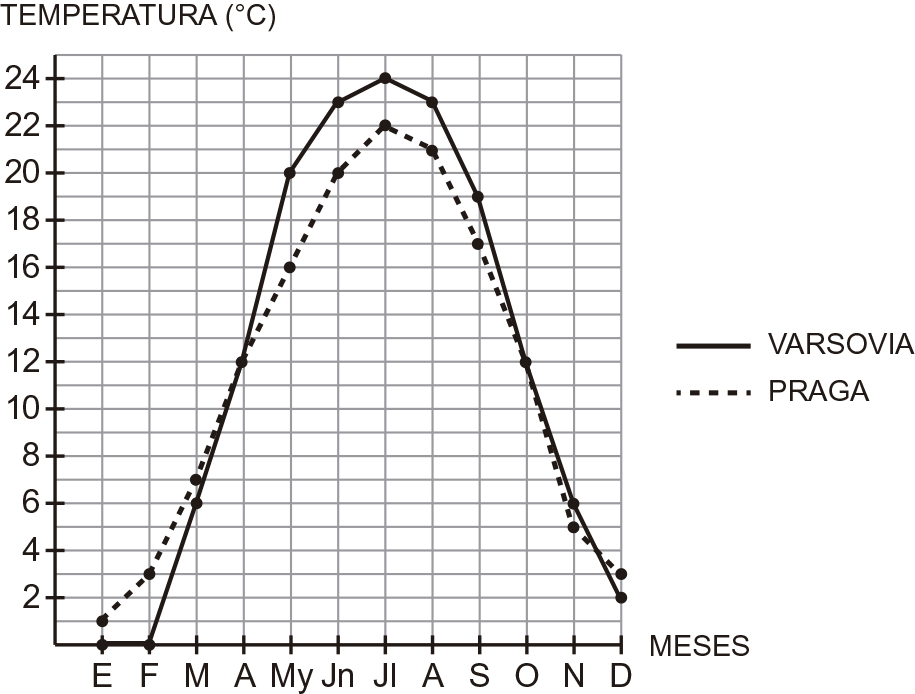
\includegraphics[]{temperaturas}
% \begin{parts}
% \part[2] ¿Entre qué mes alcanza la mayor temperatura Praga y Varsovia?
% \part[2] ¿Cuál de las dos capitales es la más fría en invierno?
% \part[2] ¿En qué mes se produce la mayor diferencia de temperatura entre ambas ciudades?
% \part[2] ¿En qué ciudad es mayor la diferencia entre la temperatura máxima y la mínima?
% \end{parts}

\
\addpoints

\end{questions}

\end{document}
